\documentclass[12pt]{article}
\usepackage{geometry}
\usepackage{graphicx}
\usepackage{float}
\usepackage{listings}

\lstset{frame=tb,
  language=bash,
  aboveskip=3mm,
  belowskip=3mm,
  showstringspaces=false,
  columns=flexible,
  basicstyle={\small\ttfamily},
  numbers=none,
  numberstyle=\tiny\color{gray},
  keywordstyle=\color{blue},
  commentstyle=\color{dkgreen},
  stringstyle=\color{mauve},
  breaklines=true,
  breakatwhitespace=true,
  tabsize=3
}
\begin{document}

\begin{flushright}
140024255\\
CS3105\\
Practical 1, Robotics
\end{flushright}

\section{Free Space Travel}
\paragraph*{Completeness}
Both the Rapidly Exploring Random Tree (RRT) robot and the Potential Fields (PF) robot exhibit completeness. With the RRT robot, it will find a path between any starting and ending point in free space, as long as the goal is within the starting GUI width and height. The starting point of the robot is allowed to be outside of the displayable region. The PF robot, on the other hand, can navigate from any arbitrary point to another arbitrary point, even outside the displayable region.

\paragraph*{Output}
As seen in Figure 1, the output of the RRT shows the entire developed tree as well as the final path outlined in green. To show the step-by-step development, the user can press the Move button. To see the final result, press the Solution button. For the PF, the user can see the development of the path (planning and execution occur in the same step) by either pressing Move for one step or Animate for all of the steps. Animate is shown with a delay in order to see the PF robot movement from one point to the next.

\paragraph*{Efficiency}
For all free space efficiency testing, the GUI size was 600,600.
For RRT efficiency testing, I set the starting point at 0,0 and the goal at 500,500 and used the final recommended settings. Specifically, the robot size was 10, the step size was 10, and the goal size was 40.
The number of moves and, since each move adds a node, the number of nodes is roughly 200 to 300 for an RRT free space simulation. The number of used nodes has a narrower range, usually between 80 and 100. The number of turns, after smoothing is usually a little less than the number of used nodes. Specifically, the number of turns fell into the range of about 80 to 90. Thus, the average number of unused nodes falls in the range 120 to 220. That means the ratio of unused to used nodes is roughly between 1.2:1 and 2.2:0.8 = 2.75:1. Length measurements fell between 800 and 1000. Adding goal bias reduced both the ratio of unused to used nodes and the length and total number of turns of paths by a significant amount. The total moves was usually around 90 to 120, and the nodes in the path was consistently 80 to 90. This means that the ratio of unused to used nodes fell drastically, almost to 0 (due to the few unused nodes) in many cases. The number of turns fell quite a bit as well, to about 70, when previously the number of turns was a bit less than the number of nodes. The length of the final path usually fell between 700 and 800. This is a decrease in length of about 100. 
For PF efficiency testing, the starting point and goal were again at 0,0 and 500,500, respectively. Recommended settings for PF were also used: a robot size of 10 and sonar size of 60.
The number of moves for the PF in free space is the same for each run, namely 20. The length of the path is always 707.106, as expected, and the number of turns is 0.

\paragraph*{Move Parameters}
To find the next move for the RRT, a random point is taken. The possible coordinate values for x and y, respectively, are from 0 to the width and 0 to the height, plus some buffer region for each. The buffer, ten percent outside of the displayable region, is needed in case the goal is at the edge of the displayable region. If this is the case, then it is much more difficult to reach as random points only reach up until the edge of the displayable region. With the buffer region, random points will reach a bit past the displayable region, making is much easier to reach goals at the edge of the displayable region.
To find the next move for the PF, the robot calculates the potential for each of the sensing points (default of 7). In the absence of obstacles, the potential is calculated solely by a formula that uses the distance from the goal. The PF then picks the sensing sample with the best (lowest) potential.

\paragraph*{Smoothing}
%%Smoothing for the RRT is relatively automatic since it uses the RRTree's nearest node method. When the step size is relatively low (10 to 15) as is recommended, the turning on the spot for the final path is limited. This is because the RRT develops paths towards the goal, and since the solution path to the goal is developed with ra
Smoothing for the PF is done by seeing the angle of movement from the current direction the robot is facing. If the next best move is the center sensor point, this means that the robot is heading straight and there is no need to smooth the path. If there is an angle between the current direction and the next move, the robot smooths the path by decreasing the length of the step. In this case, the radius of the step is the distance from the current location of the robot to the best sensor point. Depending on how far away the angle is from the straight direction, the length of the step is decreased. This happens linearly such that the step of 90 degree turns are much less than 60 degree turns, for example.

\paragraph*{Free Space Planner Superiority}
The PF robot exhibits superiority in free space in a number of aspects. It is able to find a path between any two points in free space, whereas the RRT is limited by the displayable region. Unlike the RRT, the PF does not have to do any planning. Rather, it is pulled to the goal by its attractive potential. Indeed, a lot of computation is wasted in the RRT method by calculating extra unnecessary nodes in the tree. The biggest advantage of all, of course, is that the PF robot is able to move from its starting position to the goal without any turns. Additionally, in reaching the goal in this fashion, the length of the path is reduced significantly from the wavier path of the RRT. In fact, the PF robot's path is the optimal path as it is a straight line. When adding goal bias, the PF robot's advantage is lessened by quite a bit. However, without obstacles, the straight path of the PF robot is still the optimal path.

\section{Obstacle Navigation}
\paragraph*{Output}
The output for the RRT and PF are the same as implemented in free space. The only difference is that the planning and execution of the paths have to avoid obstacles. For the RRT, the output only shows nodes that avoid any obstacles (also displayed on the screen). Thus, the output on the GUI shows the entire tree as well as the final path, except that this time there are obstacles which all nodes avoid, including the nonused ones. For the PF, the output shows the robot planning and executing its path around obstacles. The GUI displays the changing (shrinking and growing) of the sensor radius to help the user see where the possible moves are. Additionally, the sonar range and the rays from the sensors are shown to help visualize the robot detecting obstacles in its local area. Finally, the detected obstacles are highlighted red to better show the user that the robot has sensed the obstacles. The intersection points are also displayed to better show what the robot sees from its sensors.

\paragraph*{Efficiency}
Efficiency was tested once again with the parameters of the free space test.
The number of moves and, again, the number of nodes of the RRT with obstacles is a much larger range and depends on the specific obstacle course. However, for the random obstacle course, it generally falls in the 300 to 600 move range.

The PF stays in the area of 700 to 900
\paragraph*{Global Map and Local Sensing}
In addition to the move parameters described for free space, both the RRT and PF robots use additional information about the environment to avoid the obstacle. The RRT has a global map. As such, it knows if an obstacle is in the way of its next move. If so, it discards this move. The PF uses a sensor region to detect nearby obstacles. Obstacles the PF sees apply a repulsive potential that force it away. The PF also knows where the goal is without its sensors, and the goal provides an attractive potential. The RRT did not experience any problems with any of the obstacle courses. The only situation where it could not find a solution was when the robot size was too big to get past obstacles. The PF on the other hand, would get caught in local minimas and stay trapped there. F
%One other error is where the 

\paragraph*{Planner Superiority}
Although the PF is still more efficient
Overall, the RRT is a better planner when there are many obstacles present as it is much more likely that the PF robot is stuck in a local minimum. 
\paragraph*{Enhancements}
Several enhancements were added on top of the existing programs. The user is able to change many aspects of the setup, from the robot size to the step and sonar size. Further the random obstacle course gives the user a new obstacle course to test each time, with a varying number of obstacles and differing obstacle sizes. The user can also toggle between free space and obstacle course simulations, to quickly see the difference in the RRT and PF simulations.
To allow the user to better understand the PF robot's movement, the GUI displays the forward semi-circle sensors as well as the rays of the sensors to show where it might hit. Additionally, obstacles are highlighted red when they come into the obstacle's sonar range. On top of this, the GUI also displays the hit points of the rays on any obstacle. These are useful as they show the points that repulse the object, allowing a better understanding of why the robot is moving in a certain manner.
Some more usability features include allowing the user to toggle the goal bias in order to see the effect of goal bias on both free space and obstacle RRT simulations. Toggling dots also allows the user to see how random points affect the RRT tree in real time.

\section{Overview Questions}

\section{Compiling and Running}
\paragraph*{Compiling}
The files are located in the src/skynet/ subdirectory. A Makefile and ToolBox.jar are also located in this directory. The files can be compiled by running make in the same directory. 
\paragraph*{Running}
The program is run with the following command:
\begin{lstlisting}
java -cp ../:ToolBox.jar skynet.Robot
\end{lstlisting}
Optionally, there are command line arguments that change the GUI's displayable region. The usage is:
\begin{lstlisting}
java -cp ../:ToolBox.jar skynet.Robot <width pixels> <length pixels>
\end{lstlisting}

\paragraph*{Running Documentation}
Although the user is free to set whatever values for the simulation values such as robot size, sonar size, or goal coordinates, there are recommended settings in place. If the parameters are out of the recommended range, the program may exhibit unexpected and/or incorrect behavior.

The GUI provides a way for the user to initialize the setup. The robot's starting and goal position can be changed, as well as the size. The other text fields are more unique to the simulation type. Goal size and step size are only for the RRT simulation whereas sonar size is for the PF simulation. While the step and sonar size share the same text box, they only initialize the current simulation. Further, the recommended settings are changed when the simulation type is changed. The Initialize buttons for each simulation type change the type of simulation and set up the environment with the given text parameters. 

The RRT simulation has a Move and Solution button for actions. The Move button moves the RRT simulation one step. That is, the RRT tree gets another node, which is calculated from the random point. The Solution button gives the final solution for the RRT, with the final path highlighted in green. The simulation also has two other buttons that toggle simulation settings: Goal Bias and Toggle Dots. Goal bias gives the option of including goal bias to the selection of random points. More specifically, the random points are more likely to be near the goal. The Toggle Dots button allows the user to see each random dot that is used in the simulation. These are colored red. 

The PF simulation has two action buttons as well. The Move button, like in the RRT simulation, moves the PF robot on step (based on its sensor points). The Animate button moves the PF robot continuously towards the goal, animating its moves. Since the animation would be much faster if the calculations were done in real time, there is also a delay added to ensure that the animation does not move too quickly.

In order to tell the difference between which simulation is running, the action buttons for the other simulation is disabled. For example, if an RRT simulation is running, the PF simulation's Move and Animate buttons are disabled.

Finally, at the very top, there is a toggle free space button. This is used to tell both simulations whether there should be obstacles.


%figures go here
\begin{figure}
\centering
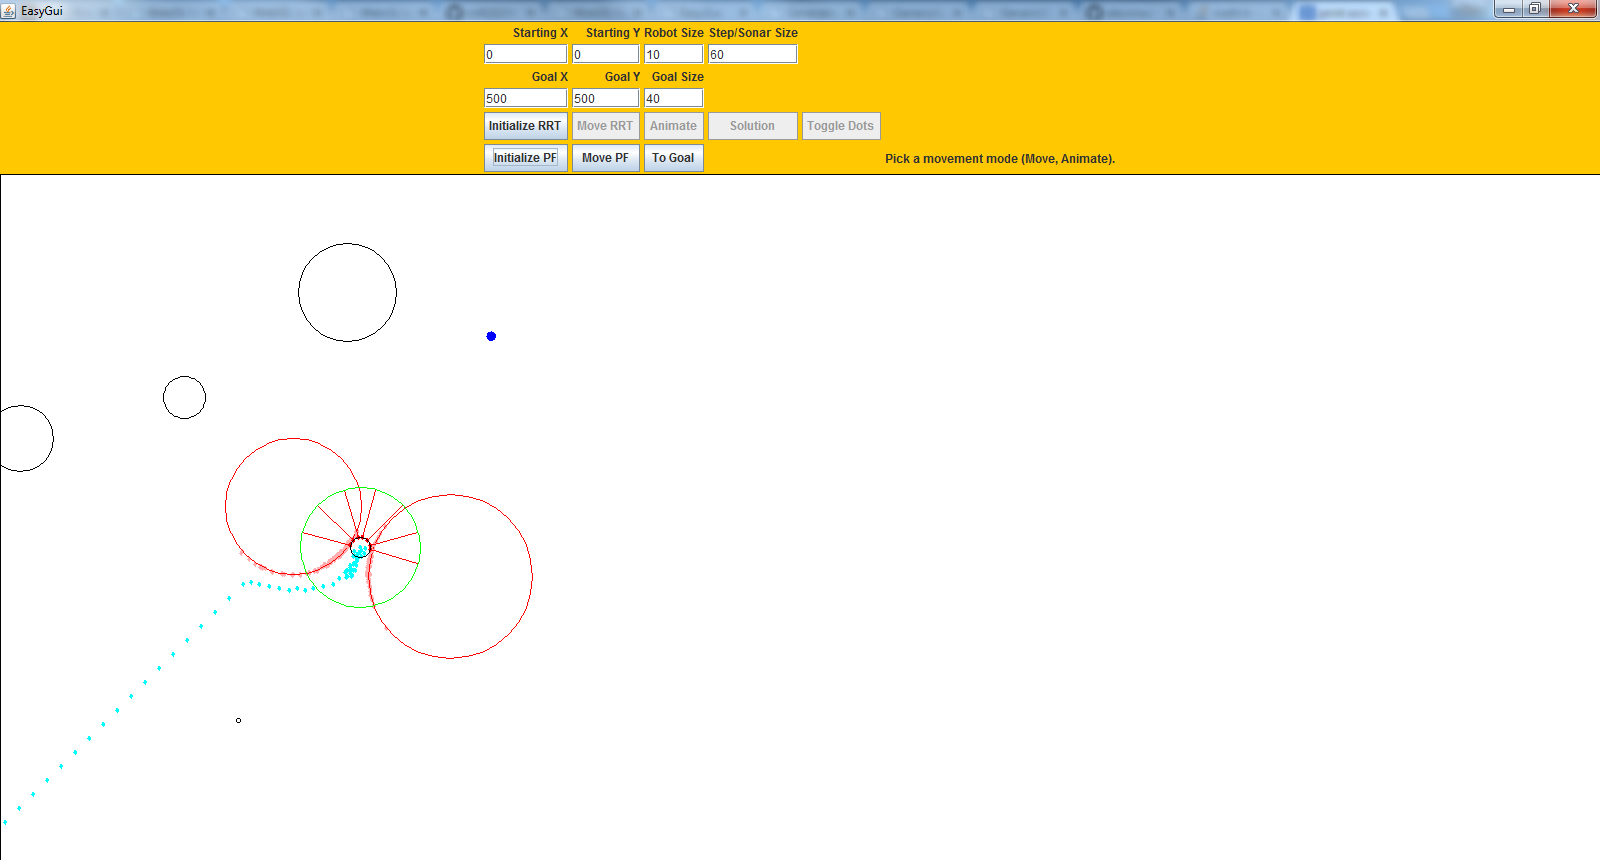
\includegraphics[width=350]{two_obstacles.png}
\caption{The PF robot stuck in a local minimum point between two obstacles.}
\end{figure}



\end{document}

